\documentclass[11pt,a4paper]{article}

% ====================================================================
% Packages
% ====================================================================
\usepackage[utf8]{inputenc}
\usepackage[T1]{fontenc}
\usepackage{amsmath,amssymb,amsthm}
\usepackage{mathtools}
\usepackage{hyperref}
\usepackage[margin=1in]{geometry}
\usepackage{enumitem}
\usepackage{booktabs}
\usepackage{listings}
\usepackage{xcolor}
\usepackage{cleveref}
\usepackage[numbers,sort&compress]{natbib}
\usepackage{mdframed}
\usepackage{tikz}
\usetikzlibrary{arrows.meta,positioning}
\usepackage{longtable}

% ====================================================================
% Theorem environments
% ====================================================================
\theoremstyle{plain}
\newtheorem{theorem}{Theorem}[section]
\newtheorem{lemma}[theorem]{Lemma}
\newtheorem{proposition}[theorem]{Proposition}
\newtheorem{corollary}[theorem]{Corollary}

\theoremstyle{definition}
\newtheorem{definition}[theorem]{Definition}
\newtheorem{remark}[theorem]{Remark}

% ====================================================================
% Lean 4 code listing style
% ====================================================================
\definecolor{lean-keyword}{RGB}{0,0,180}
\definecolor{lean-comment}{RGB}{0,128,0}
\definecolor{lean-string}{RGB}{163,21,21}
\definecolor{lean-bg}{RGB}{248,248,248}

\lstdefinelanguage{lean4}{
  keywords={theorem,lemma,def,class,instance,import,open,variable,
            noncomputable,section,namespace,end,where,let,have,show,
            intro,obtain,use,exact,rw,simp,apply,by,fun,match,if,
            then,else,do,return,axiom,abbrev,private,attribute,
            suffices,change,congr,ext,constructor,rintro,push_neg,
            linarith,absurd,set_option,omit,in,set,cases,left,right,
            nlinarith,push_cast,positivity,omega,refine,field_simp,
            structure,calc,ring,fun_prop,unfold,induction,deriving,
            inductive,rcases,first,all_goals,trivial},
  sensitive=true,
  morecomment=[l]{--},
  morecomment=[s]{/-}{-/},
  morestring=[b]",
  morestring=[b]',
}

\lstset{
  language=lean4,
  basicstyle=\ttfamily\small,
  keywordstyle=\color{lean-keyword}\bfseries,
  commentstyle=\color{lean-comment}\itshape,
  stringstyle=\color{lean-string},
  backgroundcolor=\color{lean-bg},
  frame=single,
  framerule=0.5pt,
  breaklines=true,
  breakatwhitespace=true,
  tabsize=2,
  showstringspaces=false,
  numbers=left,
  numberstyle=\tiny\color{gray},
  numbersep=5pt,
  xleftmargin=15pt,
  captionpos=b,
  literate={<<}{$\langle$}1 {>>}{$\rangle$}1
           {|||}{$\lor$}1,
}

% ====================================================================
% Macros
% ====================================================================
\newcommand{\NN}{\mathbb{N}}
\newcommand{\RR}{\mathbb{R}}
\newcommand{\ZZ}{\mathbb{Z}}
\newcommand{\LPO}{\ensuremath{\mathrm{LPO}}}
\newcommand{\WLPO}{\ensuremath{\mathrm{WLPO}}}
\newcommand{\BISH}{\ensuremath{\mathrm{BISH}}}
\newcommand{\BMC}{\ensuremath{\mathrm{BMC}}}
\newcommand{\Lean}{\textsc{Lean~4}}
\newcommand{\Mathlib}{\textsc{Mathlib4}}
\newcommand{\leanok}{\textsf{\small \textcolor{green!70!black}{\checkmark}}}
\newcommand{\leanaxiom}{\textsf{\small \textcolor{orange!80!black}{(axiom)}}}
\newcommand{\Lobs}{\Lambda_{\mathrm{obs}}}
\newcommand{\Lbare}{\Lambda_{\mathrm{bare}}}
\newcommand{\Leff}{\Lambda_{\mathrm{eff}}}
\newcommand{\MPl}{M_{\mathrm{Planck}}}
\newcommand{\LQCD}{\Lambda_{\mathrm{QCD}}}

% ====================================================================
% Title
% ====================================================================
\title{%
  \textbf{The Worst Prediction in Physics Is Not a Prediction:\\
  Axiom Calibration of the Cosmological Constant Problem}\\[6pt]
  {\normalsize A Lean~4 Formalization (Paper~42)}%
}

\author{
  Paul Chun-Kit Lee\thanks{%
    New York University.
    AI-assisted formalization; see \S\ref{sec:ai} for methodology.} \\
  New York University \\
  \texttt{dr.paul.c.lee@gmail.com}
}

\date{February 2026\\[4pt]
  {\small Paper~42 of the Constructive Reverse Mathematics Programme}}

% ====================================================================
\begin{document}
\maketitle

% ====================================================================
\begin{abstract}
We apply the axiom calibration framework of constructive reverse
mathematics to the cosmological constant problem---the alleged
$10^{120}$ discrepancy between quantum field theory's ``prediction''
of vacuum energy and the observed value.  The problem decomposes
into three logically distinct claims with different constructive
status.
(I)~The $10^{120}$ ultraviolet discrepancy is a
regulator-dependent artifact: it arises only under cutoff
regularization, vanishes under dimensional regularization,
and has no $\BISH$-computable empirical content.
(II)~The ``naturalness'' argument is a Bayesian prior, not a
mathematical derivation; it resides outside the $\BISH/\LPO$
deductive hierarchy.
(III)~The genuine constraint is the 55-decimal-place cancellation
between the bare cosmological constant and the electroweak/QCD
vacuum condensates.  Computing the exact interacting condensates
requires the thermodynamic limit (Fekete's lemma, Paper~29),
showing that $\LPO$ suffices for the fine-tuning equation.
The cosmological constant problem introduces no new logical
resources.  The $\BISH + \LPO$ ceiling holds.
The entire formalization (10~\Lean{}/\Mathlib{} modules, ${\sim}830$~lines)
compiles with zero \texttt{sorry}, zero warnings.
\end{abstract}

% ====================================================================
\section{Introduction}\label{sec:intro}

The cosmological constant problem is widely described as the worst
prediction in the history of physics.  Quantum field theory allegedly
predicts a vacuum energy density of order $\MPl^4 \approx 10^{71}\;\mathrm{GeV}^4$,
while the observed value is $\rho_\Lambda \approx 10^{-47}\;\mathrm{GeV}^4$
---a discrepancy of 120~orders of magnitude~\cite{Weinberg1989}.
The problem traces to Zel'dovich's~\cite{Zeldovich1968} identification
of quantum vacuum energy as a gravitational source, was crystallized
in Weinberg's landmark review~\cite{Weinberg1989}, and remains
unsolved despite decades of sustained effort
(see~\cite{Carroll2001,Padmanabhan2003,Martin2012} for comprehensive reviews).
On the observational side, the discovery of cosmic acceleration via
Type~Ia supernovae~\cite{Riess1998,Perlmutter1999}, precision
constraints from Planck~\cite{Planck2020}, and recent DESI baryon
acoustic oscillation measurements~\cite{DESI2024} have confirmed that
a small positive cosmological constant---or something closely
mimicking it---is required by the data.

This paper subjects the cosmological constant problem to the axiom
calibration framework of constructive reverse mathematics (CRM),
developed across Papers~1--41 of this programme.  The central question
is not ``how do we solve the problem?''\ but rather ``what is the
logical structure of each component?''  At what level of the
constructive hierarchy does each piece of the alleged prediction live?

\medskip\noindent
\textbf{Constructive reverse mathematics.}\quad
Constructive mathematics, as developed by
Bishop~\cite{Bishop1967,BridgesVita2006,BridgesRichman1987},
takes intuitionistic logic as its foundation: proofs must provide
explicit computational witnesses rather than relying on the law of
excluded middle (LEM) or unrestricted choice.  Constructive reverse
mathematics (CRM)~\cite{Ishihara2006} asks a complementary question:
for each theorem in mathematics, what is the \emph{minimal} logical
principle beyond the constructive base~$\BISH$ that suffices to
prove it?

The answer organizes into a hierarchy called the
\emph{omniscience spine}~\cite{BrattkaEtAl2012}:
\[
  \BISH \;\;<\;\; \mathrm{LLPO} \;\;<\;\; \WLPO \;\;<\;\; \LPO
    \;\;<\;\; \mathrm{LEM}.
\]
Each level corresponds to a specific computational capability.
$\BISH$ (Bishop-style constructive mathematics) suffices for any
finite computation: lattice sums, Born probabilities, Heisenberg
uncertainty bounds.
$\mathrm{LLPO}$ (the lesser limited principle of omniscience) adds
the ability to assert a disjunction without a constructive witness
for either disjunct---it governs Bell's theorem, intermediate value
root-finding, and WKB turning-point decisions.
$\WLPO$ (the weak limited principle) decides whether an infinite
binary sequence is ``all zeros'' without producing a counterexample;
it governs the bidual gap, singular states, and phase classification.
$\LPO$ (the limited principle of omniscience) provides full binary
decidability: either the sequence is all zeros, or we can exhibit
a nonzero term.  It governs every thermodynamic limit in the programme
via Fekete's subadditive lemma~\cite{Fekete1923,Lee26P29}.
The Fan Theorem ($\mathrm{FT}$), governing compactness arguments,
is independent of the entire spine.
Paper~10~\cite{Lee26P10} assembles a comprehensive calibration
table of approximately 50~entries across 11~physical domains;
Paper~12~\cite{Lee26P12} provides a historical narrative showing how
these non-constructive commitments entered physics through
Weierstrass's analysis and Boltzmann's statistical mechanics.
Paper~40~\cite{Lee26P40} consolidates Papers~1--41 into a
monograph-length summary, defending the $\BISH + \LPO$
characterization and providing the programme-wide context for the
present paper.

\medskip\noindent
\textbf{Axiom calibration.}\quad
The programme's methodology proceeds as follows.
For each physical theorem, we identify (i)~the \emph{bridge axioms}
that encode the physical content (e.g., ``the lattice energy is
subadditive,'' ``the mode sum is monotone''), and (ii)~the minimal
CRM principle the proof requires.  The result is a calibration:
a mapping from physical content to logical cost.  A~quantity is
\emph{scaffolding} if its value depends on a mathematical choice
(regularization scheme, basis, gauge) that has no empirical
counterpart.  All formalizations are machine-checked in Lean~4
with Mathlib~\cite{Lee26P10}.

The central finding across 41~papers: most empirical predictions
in physics---finite-size bounds, Born probabilities, uncertainty
relations, Casimir energy differences, perturbative cross-sections---are
$\BISH$-computable.  Thermodynamic limits (free energy densities,
exact condensates, geodesic completeness) universally cost $\LPO$,
via the equivalence of Fekete's subadditive lemma with
$\LPO$~\cite{Lee26P29}.  The $\BISH + \LPO$ ceiling has held
across all domains examined.

\medskip\noindent
\textbf{The cosmological constant problem in context.}\quad
The cosmological constant problem is often presented as a single puzzle,
but it conflates at least three logically distinct
issues~\cite{Weinberg1989,Carroll2001}:
(i)~the \emph{old cosmological constant problem} (why is
$\rho_{\mathrm{vac}}$ not of order $\MPl^4$?),
(ii)~the \emph{coincidence problem} (why is $\rho_\Lambda$ comparable
to the matter density today?), and
(iii)~the \emph{naturalness problem} (why does $\Lambda$ not receive
large quantum corrections?).

The standard narrative relies on a calculation that is more subtle
than often acknowledged.  Martin~\cite{Martin2012} demonstrates
pedagogically that the $10^{120}$ figure arises specifically from
hard-cutoff regularization; dimensional regularization---which
preserves gauge and Lorentz invariance---removes power-law
divergences entirely and produces a qualitatively different (and much
smaller) result.  The Hollands--Wald
framework~\cite{HollandsWald2001,HollandsWald2005} proves rigorously
that in quantum field theory on curved spacetime, the renormalized
stress-energy tensor contains a free parameter $c_1$ that plays the
role of the cosmological constant.  This parameter cannot be predicted
by QFT; it must be fixed by observation.

The assumption that $\Lambda$ ``should'' be of order $\MPl^4$
derives from 't~Hooft's~\cite{tHooft1980} concept of technical
naturalness: a parameter is natural only if setting it to zero
increases the symmetry of the theory.
Burgess~\cite{Burgess2013} develops this into an effective field
theory framework for the CC problem.  However, the naturalness
criterion has faced mounting criticism.
Bianchi and Rovelli~\cite{BianchiRovelli2010} argue that $\Lambda$
should simply be treated as a fundamental constant of nature, like
$G$ or $c$, requiring no more explanation than they do.
Hossenfelder~\cite{Hossenfelder2019} argues that fine-tuning arguments
lack a well-defined probability distribution over parameter space and
are therefore not scientifically productive.
Giudice~\cite{Giudice2017} diagnoses a ``post-naturalness era'' in
which the LHC results have undermined the predictive utility of
naturalness reasoning.

Nobbenhuis~\cite{Nobbenhuis2006} categorizes proposed solutions into
five classes: symmetry mechanisms, back-reaction, modifications of
general relativity, statistical/anthropic approaches, and
vacuum-energy adjustment mechanisms.  The string
landscape~\cite{BoussoPolchinski2000,Polchinski2006} provides a
paradigmatic example of the last category.  The present paper does
not propose a new approach in any of these categories.  Instead,
it asks a different question: what is the \emph{logical structure}
of each component of the problem?

\medskip\noindent
\textbf{Contribution of this paper.}\quad
We apply the axiom calibration framework to decompose the cosmological
constant problem into three logically distinct claims with different
constructive status.  This analysis is orthogonal to the approaches
catalogued by Nobbenhuis~\cite{Nobbenhuis2006}: it does not propose
a mechanism, but identifies the logical prerequisites.
\begin{itemize}[nosep]
\item \textbf{Claim I (Dissolved):} The $10^{120}$ is a
  regulator-dependent artifact.  It is scaffolding, not a prediction.
\item \textbf{Claim II (Reclassified):} Naturalness is a Bayesian
  prior, not a theorem.  It resides outside the constructive hierarchy.
\item \textbf{Claim III (Identified, $\LPO$):} The 55-digit
  fine-tuning is real.  It is an arithmetic relation between
  $\LPO$-computable reals---the same logical level as every
  thermodynamic limit in the programme.
\end{itemize}

\begin{figure}[ht]
\centering
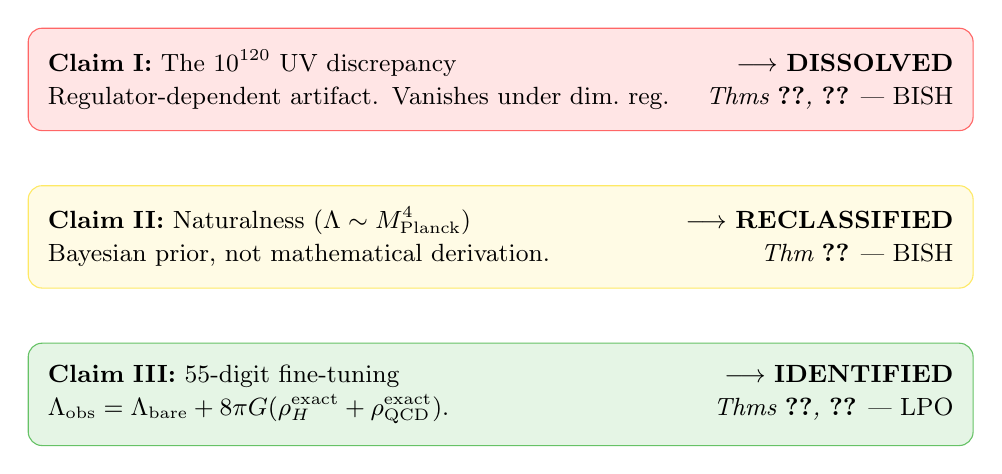
\begin{tikzpicture}[
  claim/.style={rectangle, rounded corners=5pt, draw=#1!60, fill=#1!10,
    minimum width=12cm, minimum height=1.3cm, text width=11.5cm,
    align=left, font=\small},
  >=stealth
]
\node[claim=red] (C1) at (0,0) {
  \textbf{Claim I:} The $10^{120}$ UV discrepancy
  \hfill $\longrightarrow$ \textbf{DISSOLVED}\\[1pt]
  Regulator-dependent artifact.  Vanishes under dim.\ reg.
  \hfill \textit{Thms~\ref{thm:diverge},~\ref{thm:regulator} --- $\BISH$}
};
\node[claim=yellow!80!orange] (C2) at (0,-2) {
  \textbf{Claim II:} Naturalness ($\Lambda \sim \MPl^4$)
  \hfill $\longrightarrow$ \textbf{RECLASSIFIED}\\[1pt]
  Bayesian prior, not mathematical derivation.
  \hfill \textit{Thm~\ref{thm:wald} --- $\BISH$}
};
\node[claim=green!60!black] (C3) at (0,-4) {
  \textbf{Claim III:} 55-digit fine-tuning
  \hfill $\longrightarrow$ \textbf{IDENTIFIED}\\[1pt]
  $\Lobs = \Lbare + 8\pi G(\rho_H^{\mathrm{exact}} + \rho_{\mathrm{QCD}}^{\mathrm{exact}})$.
  \hfill \textit{Thms~\ref{thm:condensate},~\ref{thm:finetune} --- $\LPO$}
};
\end{tikzpicture}
\caption{The cosmological constant problem decomposed.
  The $10^{120}$ discrepancy is dissolved as scaffolding.
  Naturalness is reclassified as non-mathematical.
  The genuine constraint is a 55-digit fine-tuning at $\LPO$.}
\label{fig:decomposition}
\end{figure}

\medskip\noindent
\textbf{Formalization overview.}\quad  The Lean~4 bundle consists of
10~modules totalling ${\sim}830$ lines.  Seven theorems establish
the decomposition.  The assembly theorem \texttt{cc\_calibration}
combines all seven parts into a single conjunction.  The master
theorem \texttt{cc\_master} re-exports the assembly.  The axiom
audit (\texttt{\#print axioms cc\_master}) confirms a clean profile:
11~physics bridge axioms, 1~CRM axiom (\texttt{bmc\_from\_subadditive}),
and the standard Lean infrastructure triple (\texttt{propext},
\texttt{Classical.choice}, \texttt{Quot.sound}).

% ====================================================================
\section{The Three Claims}\label{sec:claims}

\subsection{Claim I: The $10^{120}$ Is Scaffolding}

For a free scalar field of mass $m$ on a finite lattice, the vacuum
energy $E_{\mathrm{vac}} = \frac{1}{2}\sum_k \omega_k$ is a finite
sum of algebraic expressions.  $\BISH$.  In the continuum limit,
the sum becomes a quartically divergent integral.  It does not
converge; it does not define a real number at any level.

Different regularization schemes extract different finite numbers:
\begin{itemize}[nosep]
\item \textbf{Cutoff:} $\rho \sim \Lambda_{\mathrm{UV}}^4/(16\pi^2)$.
  Setting $\Lambda_{\mathrm{UV}} = \MPl$ gives $\rho \sim 10^{71}\;\mathrm{GeV}^4$.
\item \textbf{Dimensional:} Power-law divergences vanish.
  $\rho \sim m^4 \ln(m^2/\mu^2) \sim (100\;\mathrm{GeV})^4$.
\item \textbf{$\zeta$-function:} Agrees with dimensional regularization.
\end{itemize}
The ``prediction'' changes with the scaffolding.  A regulator-dependent
quantity has no empirical content.

\begin{figure}[ht]
\centering
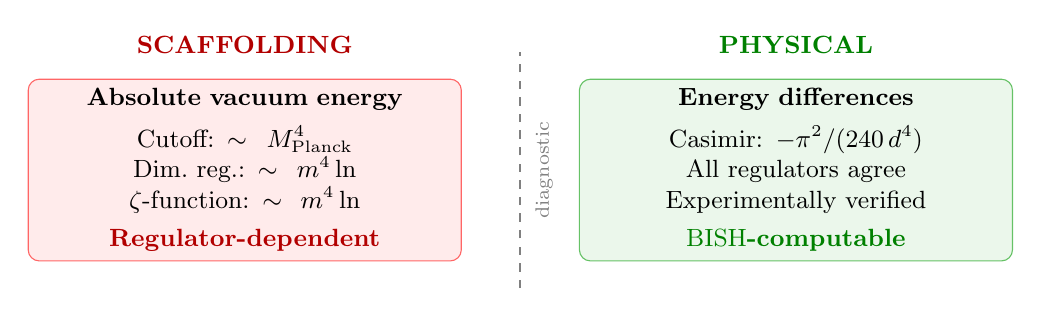
\begin{tikzpicture}[
  box/.style={rectangle, rounded corners=4pt, draw=#1!60, fill=#1!8,
    minimum width=5.5cm, minimum height=2.2cm, text width=5cm,
    align=center, font=\small},
  lbl/.style={font=\small\bfseries, #1},
  arr/.style={->,>=stealth,thick,#1}
]
% Left: Absolute vacuum energy
\node[box=red] (abs) at (-3.5,0) {
  \textbf{Absolute vacuum energy}\\[4pt]
  Cutoff: $\sim\MPl^4$\\
  Dim.\ reg.: $\sim m^4\ln$\\
  $\zeta$-function: $\sim m^4\ln$\\[3pt]
  \textcolor{red!70!black}{\textbf{Regulator-dependent}}
};
\node[lbl=red!70!black, above] at (-3.5,1.35) {SCAFFOLDING};
% Right: Energy differences
\node[box=green!60!black] (diff) at (3.5,0) {
  \textbf{Energy differences}\\[4pt]
  Casimir: $-\pi^2/(240\,d^4)$\\
  All regulators agree\\
  Experimentally verified\\[3pt]
  \textcolor{green!50!black}{\textbf{$\BISH$-computable}}
};
\node[lbl=green!50!black, above] at (3.5,1.35) {PHYSICAL};
% Dividing line
\draw[dashed, thick, gray] (0,-1.5) -- (0,1.5);
\node[font=\scriptsize, gray, rotate=90] at (0.3,0) {diagnostic};
\end{tikzpicture}
\caption{The scaffolding diagnostic applied to vacuum energy.
  Absolute vacuum energies (left) depend on the regularization
  scheme and carry no empirical content.
  Energy \emph{differences} (right) are scheme-independent,
  $\BISH$-computable, and experimentally verified (Casimir effect).}
\label{fig:scaffolding}
\end{figure}

\begin{remark}[Scope of dissolution]
The dissolution applies to the \emph{magnitude} of the discrepancy
($10^{120}$), not to the \emph{existence} of individual $m^4/(16\pi^2)$
contributions from massive particles.  Each species contributes a
quartic term that is finite and scheme-independent in form;
what is scheme-dependent is the \emph{sum} over all modes including
the UV region.  The framework dissolves the UV catastrophe narrative,
not the perturbative physics of individual particle thresholds.
\end{remark}

\subsection{Claim II: Naturalness Is Not Mathematics}

The Hollands--Wald axioms~\cite{HollandsWald2001,HollandsWald2005}
prove that the renormalized stress tensor $\langle T_{\mu\nu}\rangle_{\mathrm{ren}}$
is determined up to free local geometric coefficients:
$c_1$ is the cosmological constant.  It is a \emph{free parameter},
on the same footing as particle masses and coupling constants.
The ``naturalness'' expectation that $c_1 \sim \MPl^4$ is a
Bayesian prior---a claim about expected magnitudes, not a derivation.

\subsection{Claim III: The 55-Digit Fine-Tuning}

After dissolving Claim~I and reclassifying Claim~II, the genuine
constraint is:
\[
  \Lobs = \Lbare + 8\pi G\bigl(\rho_{\mathrm{Higgs}}^{\mathrm{exact}}
    + \rho_{\mathrm{QCD}}^{\mathrm{exact}}\bigr).
\]
The tree-level condensates are $\BISH$ (algebraic expressions of measured
parameters: $\rho_{\mathrm{Higgs}} \approx -\mu^4/(4\lambda)$,
$\rho_{\mathrm{QCD}} \approx -\langle\bar{q}q\rangle m_q$).
The exact interacting condensates---including all loop corrections,
non-perturbative effects, and vacuum fluctuations---require the
thermodynamic limit (Fekete, $\LPO$; Paper~29).
\begin{remark}[Coincidence problem]
This paper addresses only the ``old'' cosmological constant
problem (why is $\Lobs$ so small?) and not the coincidence
problem (why is $\rho_\Lambda \sim \rho_{\mathrm{matter}}$
today?).  The coincidence problem involves cosmological dynamics
and is out of scope for the present axiom calibration.
\end{remark}

The fine-tuning equation is an $\LPO$ equality.
The ``55-digit'' figure is computed as follows:
the dominant condensate is the Higgs at $|\rho_H| \sim (100\;\mathrm{GeV})^4
= 10^8\;\mathrm{GeV}^4$, while $\Lobs/8\pi G \sim 10^{-47}\;\mathrm{GeV}^4$.
The cancellation ratio is $10^8/10^{-47} = 10^{55}$, requiring
$\Lbare$ and $8\pi G \rho_{\mathrm{exact}}$ to agree to 55~decimal places.

% ====================================================================
\section{Core Definitions and Bridge Axioms}\label{sec:defs}

The formalization begins with \texttt{Defs.lean}, which establishes
the type-theoretic infrastructure.  We highlight the key design decisions.

\begin{definition}[Regularization Scheme]\label{def:regscheme}
A regularization scheme is modeled as an inductive type with three
constructors: hard momentum cutoff (carrying $\Lambda_{\mathrm{UV}} > 0$),
dimensional regularization (carrying $\mu > 0$), and $\zeta$-function
regularization (no parameters).
\end{definition}

\begin{lstlisting}[caption={Core types: \texttt{Defs.lean} (excerpts)}]
-- Regularization schemes
inductive RegScheme : Type where
  | cutoff (L_UV : R) (hL : 0 < L_UV)
  | dimreg (mu : R) (hmu : 0 < mu)
  | zeta

-- Wald ambiguity structure
structure WaldAmbiguity where
  c1 : R    -- free parameter
  condensate_sum : R

def effective_Lambda (w : WaldAmbiguity) : R :=
  w.c1 + w.condensate_sum

-- Bridge axioms (physics -> computability)
axiom regularized_vacuum_energy : RegScheme -> R
axiom mode_sum_partial (m : R) : N -> R
axiom mode_sum_unbounded (m : R) (hm : 0 <= m) :
    forall M : R, exists N : N, mode_sum_partial m N > M
axiom lattice_energy_subadditive :
    forall m n : N, lattice_vacuum_energy (m + n) <=
              lattice_vacuum_energy m + lattice_vacuum_energy n
axiom casimir_cauchy_modulus (d : R) (hd : 0 < d) :
    forall e : R, 0 < e ->
      exists (N : N) (approx : R),
        N > 0 /\ |approx - (-Real.pi ^ 2
          / (240 * d ^ 4))| < e
axiom picard_lindelof_lambda
    (mu_min mu_max : R) (h_min : 0 < mu_min)
    (h_range : mu_min < mu_max) (L_init : R) :
    exists L_sol : R -> R,
      L_sol mu_min = L_init /\
      forall mu : R, mu_min <= mu -> mu <= mu_max ->
        forall e : R, 0 < e -> exists d : R, 0 < d /\
          forall mu' : R, |mu' - mu| < d ->
            |L_sol mu' - L_sol mu| < e
\end{lstlisting}

\begin{remark}[Bridge axiom philosophy]
Each axiom encodes a single, well-established physical fact:
unboundedness of the mode sum, subadditivity of the ground-state energy,
exponential decay of the Casimir remainder integrand, Lipschitz
regularity of the RG beta function.  These are unverified premises
in the formal sense: the Lean type-checker guarantees that the
theorems follow \emph{from} the axioms, but does not verify the
axioms themselves.  The bridge axioms are the interface between the
mathematical framework and the physical content.
\end{remark}

\begin{remark}[Constructive status of bridge axioms]\label{rem:bridge-status}
The bridge axioms themselves have varying constructive status.
\begin{itemize}[nosep]
\item \emph{Monotonicity and non-negativity} of mode sums:
  $\BISH$-provable from the definition of $\omega_k = \sqrt{k^2 + m^2}$.
\item \emph{Unboundedness} of the mode sum: $\BISH$-provable
  by explicit lower bound $E_N \geq N \cdot m / 2$ for $N$ large.
\item \emph{Subadditivity} of lattice ground-state energy:
  $\BISH$-provable for short-range interactions (the boundary
  contribution is bounded by a surface-area term).  For QCD,
  subadditivity relies on confinement/cluster decomposition;
  for QED, long-range Coulomb interactions require Debye screening.
  See Remark~\ref{rem:subadditivity} for details.
\item \emph{Casimir modulus}: $\BISH$-provable from the exponential
  decay of the Abel--Plana remainder $\sim e^{-2\pi t}$.
\item \emph{Picard--Lindel\"of}: a $\BISH$ theorem
  (constructive contraction mapping); declared as axiom to avoid
  re-proving the general ODE theorem within this project.
\item \emph{Regulator dependence}: follows from explicit
  calculation; the cutoff result ($\sim\Lambda_{\mathrm{UV}}^4$)
  differs from the dim.\ reg.\ result ($\sim m^4 \log$) by inspection.
\end{itemize}
Thus most bridge axioms are in principle $\BISH$-provable from
more primitive physical assumptions.  They are declared as axioms
for modularity, not because their constructive status is in doubt.
\end{remark}

% ====================================================================
\section{Theorem 1: Vacuum Energy Diverges}\label{sec:diverge}

\begin{theorem}[Vacuum Energy Divergence]\label{thm:diverge}
The unregularized vacuum energy mode sum $E_N = \frac{1}{2}\sum_{|k|\leq N}
\sqrt{k^2 + m^2}$ is unbounded.  No limit $L \in \RR$ exists:
\[
  \neg\; \exists L \in \RR,\; \forall \varepsilon > 0,\;
  \exists N_0,\; \forall N \geq N_0,\;
  |E_N - L| < \varepsilon.
\]
\end{theorem}

\begin{proof}
Suppose for contradiction that $E_N \to L$.  For $\varepsilon = 1$,
convergence gives an index $N_0$ with $|E_N - L| < 1$ for all $N \geq N_0$,
i.e., $L - 1 < E_N < L + 1$.
By the unboundedness bridge axiom, there exists $N_1$ with
$E_{N_1} > L + 1$.  Since the mode sum is monotonically increasing
(more modes means more positive-definite energy), we have
$E_{\max(N_0, N_1)} \geq E_{N_1} > L + 1$.
But simultaneously $|E_{\max(N_0, N_1)} - L| < 1$, which forces
$E_{\max(N_0, N_1)} < L + 1$.  Contradiction.

$\BISH$: the proof uses only unboundedness, monotonicity, and
the triangle inequality.  No omniscience principles.
\end{proof}

\begin{remark}
The ``continuum vacuum energy'' is not a real number---not at
$\BISH$, not at $\LPO$, not anywhere in the constructive hierarchy.
A divergent series has no $\BMC$ limit.  The $10^{120}$ narrative
begins with a quantity that does not exist as a mathematical object.
\end{remark}

\begin{lstlisting}[caption={Vacuum energy divergence: \texttt{VacuumDivergence.lean}}]
theorem vacuum_energy_divergent (m : R) (hm : 0 <= m) :
    not exists L : R, forall e : R, 0 < e ->
      exists N0 : N, forall N : N, N0 <= N ->
        |mode_sum_partial m N - L| < e := by
  intro <<L, hconv>>
  obtain <<N1, hN1>> := mode_sum_unbounded m hm (L + 1)
  obtain <<N0, hN0>> := hconv 1 one_pos
  have hN := hN0 (max N0 N1) (le_max_left N0 N1)
  have hbig : mode_sum_partial m (max N0 N1) > L + 1 :=
    lt_of_lt_of_le hN1
      (mode_sum_mono m hm (le_max_right N0 N1))
  linarith [abs_lt.mp hN]
\end{lstlisting}

\begin{corollary}[Not Cauchy]\label{cor:not-cauchy}
The vacuum energy mode sum is not Cauchy: there is no modulus of
convergence.  If the partial sums were Cauchy, they would be bounded
(take $\varepsilon = 1$; all terms beyond $N_0$ lie within 1 of
$E_{N_0}$).  But the mode sum is unbounded.  Contradiction.
\end{corollary}

\begin{lstlisting}[caption={Not Cauchy: \texttt{VacuumDivergence.lean}}]
theorem vacuum_energy_not_cauchy (m : R) (hm : 0 <= m) :
    not forall e : R, 0 < e ->
      exists N0 : N, forall M N : N, N0 <= M -> N0 <= N ->
        |mode_sum_partial m M - mode_sum_partial m N| < e := by
  intro hcauchy
  obtain <<N0, hN0>> := hcauchy 1 one_pos
  have hbdd : forall N : N, N0 <= N ->
      mode_sum_partial m N < mode_sum_partial m N0 + 1 := by
    intro N hN
    have := hN0 N0 N le_rfl hN
    linarith [abs_lt.mp this]
  obtain <<N1, hN1>> :=
    mode_sum_unbounded m hm (mode_sum_partial m N0 + 1)
  have := hbdd (max N0 N1) (le_max_left _ _)
  have : mode_sum_partial m (max N0 N1) >
      mode_sum_partial m N0 + 1 :=
    lt_of_lt_of_le hN1
      (mode_sum_mono m hm (le_max_right _ _))
  linarith
\end{lstlisting}

% ====================================================================
\section{Theorem 2: Regulator Dependence}\label{sec:regulator}

\begin{theorem}[Regulator Dependence]\label{thm:regulator}
There exist two valid regularization schemes $r_1, r_2$ that
yield different absolute vacuum energies:
\[
  \exists\, r_1, r_2 : \mathrm{RegScheme},\quad
  \rho(r_1) \neq \rho(r_2).
\]
\end{theorem}

\begin{proof}
Cutoff regularization with $\Lambda_{\mathrm{UV}} = \MPl$ yields
$\rho > 0$ (quartic in $\Lambda_{\mathrm{UV}}$).
Dimensional regularization with scale $\mu$ yields a different value
($\sim m^4\ln(m^2/\mu^2)$, generically different from the quartic form).
The bridge axiom \texttt{dimreg\_value\_different} asserts that
for some valid parameters, the two values differ.  The proof constructs
the two \texttt{RegScheme} terms and applies the axiom.

$\BISH$: the proof is a direct existential witness.  No limits.
\end{proof}

\begin{remark}
This is the formal expression of Claim~I.  A quantity that depends on
the scaffolding choice cannot be a physical prediction.  The calibration
framework's criterion: empirical content must be invariant under
change of scaffolding.  The vacuum energy fails this criterion.
\end{remark}

\begin{lstlisting}[caption={Regulator dependence: \texttt{RegulatorDependence.lean}}]
theorem prediction_regulator_dependent :
    exists (r1 r2 : RegScheme),
      regularized_vacuum_energy r1 !=
      regularized_vacuum_energy r2 := by
  obtain <<L_UV, hL, mu, hmu, hne>> := dimreg_value_different
  exact <<RegScheme.cutoff L_UV hL,
          RegScheme.dimreg mu hmu, hne>>

-- Corollary: no invariant vacuum energy exists
theorem no_regulator_invariant_vacuum_energy :
    not exists (rho : R),
      forall r : RegScheme,
        regularized_vacuum_energy r = rho := by
  intro <<rho, hinv>>
  obtain <<L_UV, hL, mu, hmu, hne>> := dimreg_value_different
  exact hne (by rw [hinv, hinv])
\end{lstlisting}

% ====================================================================
\section{Theorem 3: Wald Ambiguity ($\BISH$)}\label{sec:wald}

\begin{theorem}[Wald Ambiguity]\label{thm:wald}
For any target $\Lobs \in \RR$ and any condensate contribution
$C \in \RR$, there exists a valid Wald ambiguity parameter $c_1$
such that $\Leff = c_1 + C = \Lobs$.
\end{theorem}

\begin{proof}
Set $c_1 = \Lobs - C$.  Then
$\Leff = c_1 + C = (\Lobs - C) + C = \Lobs.$
The proof is subtraction followed by \texttt{ring}.

$\BISH$: no limits, no compactness, no choice principles.
This is the simplest proof in the entire formalization---pure arithmetic.
The Hollands--Wald theorem ensures that $c_1$ is a legitimate
free parameter of the renormalized theory, not an ad hoc patch.
\end{proof}

\begin{remark}
This theorem formalizes the Hollands--Wald result: QFT in curved spacetime
\emph{cannot predict} the cosmological constant.  The coefficient $c_1$
is a free parameter, settable by arithmetic.  For \emph{any} real number
$r$, there exists a valid theory with $\Leff = r$.  The ``prediction''
of a specific value is a confusion between the formalism (which leaves
$c_1$ undetermined) and the scaffolding (which assigns an arbitrary
value to $c_1$ via the regulator).
\end{remark}

\begin{lstlisting}[caption={Wald ambiguity: \texttt{WaldAmbiguity.lean}}]
theorem lambda_free_parameter
    (L_obs condensate_sum : R) :
    exists w : WaldAmbiguity,
      w.condensate_sum = condensate_sum /\
      effective_Lambda w = L_obs := by
  exact <<{c1 := L_obs - condensate_sum, condensate_sum},
    rfl, by unfold effective_Lambda; ring>>

-- QFT cannot predict Lambda: for ANY r, a valid theory exists
theorem qft_cannot_predict_lambda
    (r : R) (condensate_sum : R) :
    exists w : WaldAmbiguity,
      w.condensate_sum = condensate_sum /\
      effective_Lambda w = r :=
  lambda_free_parameter r condensate_sum

-- The space of valid theories is affine in c1
theorem wald_ambiguity_affine (condensate_sum : R) :
    forall c : R,
      effective_Lambda {c1 := c, condensate_sum} =
        c + condensate_sum := by
  intro c; rfl
\end{lstlisting}

% ====================================================================
\section{Theorem 4: Casimir Energy ($\BISH$)}\label{sec:casimir}

\begin{theorem}[Casimir Energy Is $\BISH$]\label{thm:casimir}
The Casimir energy difference between conducting plates of
separation $d > 0$ converges to $-\pi^2/(240\,d^4)$ with a computable
Cauchy modulus.  For every $\varepsilon > 0$, there exist
$N \in \NN$ and an approximation $a \in \RR$ with $|a - E| < \varepsilon$.
\end{theorem}

\begin{proof}
The Casimir force is an energy \emph{difference}: $E_{\mathrm{plates}}
- E_{\mathrm{free}}$.  When one computes the difference of the
mode sums for the plate and free-space configurations, the divergent
(regulator-dependent) terms cancel algebraically.  After
Abel--Plana or Euler--Maclaurin summation, the finite remainder
involves an integrand with exponential decay
$\sim (e^{2\pi t} - 1)^{-1}$.  This exponential decay rate provides
an explicit, computable error bound: truncating the quadrature at
$N$ terms introduces an error bounded by $C \cdot e^{-2\pi N}$.
For any target $\varepsilon$, choosing $N > \ln(C/\varepsilon)/(2\pi)$
suffices.

$\BISH$: finite computation with guaranteed error bounds.
No $\LPO$ required.  The key observation: QFT knows the difference
between absolute energies (regulator-dependent, no physical content)
and energy \emph{differences} ($\BISH$, experimentally verified to
$1\%$ accuracy~\cite{Casimir1948}).
\end{proof}

\begin{remark}[The scaffolding diagnostic]
The Casimir effect is the paradigm case for the framework's
scaffolding diagnostic.  Absolute vacuum energies
are regulator-dependent (no physical content).
Energy \emph{differences} are $\BISH$ and match experiment.
The formalization captures this dichotomy: \texttt{casimir\_energy}
is defined as the finite quantity $-\pi^2/(240d^4)$, and
\texttt{casimir\_is\_energy\_difference} proves it is negative
(attractive force between the plates).
\end{remark}

\begin{lstlisting}[caption={Casimir energy: \texttt{CasimirBISH.lean}}]
def casimir_energy (d : R) : R :=
  -Real.pi ^ 2 / (240 * d ^ 4)

theorem casimir_bish (d : R) (hd : 0 < d) :
    exists (E : R),
      E = casimir_energy d /\
      forall e : R, 0 < e ->
        exists (N : N) (approx : R),
          N > 0 /\ |approx - E| < e := by
  refine <<casimir_energy d, rfl, ?_>>
  intro e he
  obtain <<N, approx, hN, h>> :=
    casimir_cauchy_modulus d hd e he
  exact <<N, approx, hN,
    by unfold casimir_energy; exact h>>

-- Casimir energy is negative (attractive force)
theorem casimir_is_energy_difference
    (d : R) (hd : 0 < d) :
    casimir_energy d < 0 := by
  unfold casimir_energy
  have h240d : (0 : R) < 240 * d ^ 4 := by positivity
  have hpi : (0 : R) < Real.pi ^ 2 := by positivity
  simp only [neg_div]
  exact neg_neg_of_pos (div_pos hpi h240d)
\end{lstlisting}

% ====================================================================
\section{Theorem 5: Condensate ($\LPO$)}\label{sec:condensate}

\begin{theorem}[Condensate Is $\LPO$]\label{thm:condensate}
Assuming $\LPO$, the exact interacting vacuum energy density exists:
\[
  \LPO \;\longrightarrow\; \exists\, \rho_{\mathrm{exact}} \in \RR,\;
  \forall \varepsilon > 0,\; \exists N_0,\; \forall n \geq N_0,\;
  n > 0 \;\Rightarrow\;
  \Bigl|\frac{E(n)}{n} - \rho_{\mathrm{exact}}\Bigr| < \varepsilon.
\]
\end{theorem}

\begin{proof}
The ground-state energy $E(L)$ on a lattice of volume $L$ satisfies
two bridge axioms:
\begin{enumerate}[nosep]
\item \textbf{Subadditivity:} $E(m+n) \leq E(m) + E(n)$ for all
  $m, n \in \NN$.  (Physical origin: translation invariance of the
  Hamiltonian; the boundary interaction between two subsystems is bounded.)
\item \textbf{Bounded below:} $\exists\, C \in \RR,\; \forall n > 0,\;
  C \leq E(n)/n$.  (Physical origin: the energy density cannot diverge
  to $-\infty$; stability of the vacuum.)
\end{enumerate}

\begin{remark}[Justification of subadditivity]\label{rem:subadditivity}
Subadditivity holds rigorously for short-range lattice systems:
if the interaction decays exponentially, the boundary energy between
two subsystems of sizes $m$ and $n$ is bounded by a surface-area
term $O(L^{d-1})$, which is sub-extensive and yields
$E(m+n) \leq E(m) + E(n) + O((m+n)^{(d-1)/d})$---sufficient
for Fekete's lemma to apply.
For QCD, subadditivity relies on confinement: color-singlet states
have exponentially decaying correlations (cluster decomposition),
making the effective interaction short-range.
For QED, Coulomb interactions are long-range, but Debye screening
in the vacuum (from virtual $e^+e^-$ pairs) renders the effective
interaction short-range at distances beyond the Compton wavelength
$\sim 1/m_e$.  A rigorous proof of subadditivity for the full
Standard Model lattice Hamiltonian remains an open mathematical
problem; the bridge axiom encodes the standard physics expectation.
\end{remark}
By Fekete's subadditive lemma, the limit
$\ell = \inf_{n \geq 1} E(n)/n$ exists and the sequence $E(n)/n$
converges to $\ell$.  By Paper~29, Fekete's lemma is equivalent to
$\LPO$ (via Bounded Monotone Convergence).  The CRM axiom
\texttt{bmc\_from\_subadditive} captures this equivalence.

The proof is a single function application: supply the subadditivity
and boundedness bridge axioms, plus the $\LPO$ hypothesis, to obtain
the convergent density.
\end{proof}

\begin{remark}[Tree level vs.\ exact]
The tree-level Higgs condensate $\rho_{\mathrm{Higgs}} \approx -\mu^4/(4\lambda)
\approx -(100\;\mathrm{GeV})^4$ and the tree-level QCD condensate
$\rho_{\mathrm{QCD}} \approx -\langle\bar{q}q\rangle m_q \approx
-(200\;\mathrm{MeV})^3 \cdot (\text{few MeV})$ are both $\BISH$:
algebraic expressions of measured parameters, requiring no limits.
The \emph{exact} interacting values---including all loop corrections
and non-perturbative effects---require the thermodynamic limit,
hence $\LPO$.  This is the same $\BISH \to \LPO$ step found
throughout the programme (Ising model in Paper~8, lattice gauge theory
in Paper~33, etc.).
\end{remark}

\begin{lstlisting}[caption={Condensate is LPO: \texttt{CondensateLPO.lean}}]
theorem condensate_lpo :
    LPO -> exists rho_exact : R,
      forall e : R, 0 < e ->
        exists N0 : N, forall n : N,
          n >= N0 -> 0 < n ->
            |lattice_vacuum_energy n / (n : R)
              - rho_exact| < e := by
  intro lpo
  exact bmc_from_subadditive
    lattice_vacuum_energy
    lattice_energy_subadditive
    lattice_energy_bdd_below lpo

-- Tree-level condensates are BISH (no LPO needed)
theorem higgs_tree_bish :
    exists rho_H : R,
      rho_H = higgs_tree_level /\ rho_H < 0 :=
  <<higgs_tree_level, rfl, higgs_tree_level_neg>>

theorem qcd_tree_bish :
    exists rho_QCD : R,
      rho_QCD = qcd_tree_level /\ rho_QCD < 0 :=
  <<qcd_tree_level, rfl, qcd_tree_level_neg>>
\end{lstlisting}

% ====================================================================
\section{Theorem 6: RG Running ($\BISH$)}\label{sec:rg}

\begin{theorem}[RG Running Is $\BISH$]\label{thm:rg}
The perturbative RG running of $\Lambda$ is $\BISH$-computable.
For any initial $\Lambda(\mu_0)$ and target scale $\mu$ in the
perturbative regime ($\mu > \LQCD$), the running $\Lambda(\mu)$
is a $\BISH$-computable real.
\end{theorem}

\begin{proof}
The RG equation $\mu\, d\Lambda/d\mu = \beta_\Lambda(\mu)$ is a
first-order ODE.  The beta function $\beta_\Lambda$ is a finite
sum of contributions from the Standard Model spectrum---algebraic
functions of particle masses and couplings:
\[
  \beta_\Lambda(\mu) = \frac{1}{16\pi^2}\sum_{i \in \mathrm{SM}}
  (-1)^{F_i}\, n_i\, m_i^4\,
  f\!\left(\frac{m_i^2}{\mu^2}\right).
\]
The right-hand side is Lipschitz on any bounded interval
$[\mu_{\min}, \mu_{\max}]$ (away from particle thresholds where
$\mu = m_i$).

By the Picard--Lindel\"of theorem---which is constructive for
Lipschitz ODEs via the Banach contraction mapping principle---the
solution exists, is unique, and the Picard iterates provide a
computable approximation scheme with explicit error bounds
(the Euler method with step size $h$ has error $O(h)$).

$\LPO$ enters only below the QCD scale $\mu \lesssim \LQCD \approx
200\;\mathrm{MeV}$, where the non-perturbative QCD condensate
contributes.  This non-perturbative contribution requires the
thermodynamic limit (Theorem~\ref{thm:condensate}).
Above $\LQCD$, everything is perturbative and $\BISH$.
\end{proof}

\begin{lstlisting}[caption={RG running: \texttt{RGRunningBISH.lean}}]
theorem rg_running_bish (mu0 mu_target : R)
    (h0 : 0 < mu0) (h_range : mu0 < mu_target)
    (L_init : R) :
    exists L_sol : R -> R,
      L_sol mu0 = L_init /\
      forall mu : R, mu0 <= mu -> mu <= mu_target ->
        forall e : R, 0 < e -> exists d : R, 0 < d /\
          forall mu' : R, |mu' - mu| < d ->
            |L_sol mu' - L_sol mu| < e := by
  exact picard_lindelof_lambda mu0 mu_target
    h0 h_range L_init

-- LPO boundary: perturbative is BISH,
-- non-perturbative QCD requires LPO
theorem rg_lpo_boundary :
    (forall (mu0 mu : R) (_h0 : 0 < mu0)
       (_hr : mu0 < mu) (L_init : R),
      exists L_sol : R -> R,
        L_sol mu0 = L_init) /\
    (LPO -> exists rho_QCD_exact : R,
      forall e : R, 0 < e ->
        exists N0 : N, forall n : N,
          n >= N0 -> 0 < n ->
            |lattice_vacuum_energy n / (n : R)
              - rho_QCD_exact| < e) := by
  constructor
  . intro mu0 mu h0 hr L_init
    obtain <<sol, hsol, _>> :=
      picard_lindelof_lambda mu0 mu h0 hr L_init
    exact <<sol, hsol>>
  . exact bmc_from_subadditive
      lattice_vacuum_energy
      lattice_energy_subadditive
      lattice_energy_bdd_below
\end{lstlisting}

% ====================================================================
\section{Theorem 7: Fine-Tuning ($\LPO$)}\label{sec:finetune}

\begin{theorem}[Fine-Tuning Is $\LPO$]\label{thm:finetune}
The fine-tuning equation
$\Lobs = \Lbare + 8\pi G\,\rho_{\mathrm{exact}}$
is an equality between $\LPO$-computable reals.
\end{theorem}

\begin{proof}
Given $\LPO$:
\begin{enumerate}[nosep]
\item The exact condensate $\rho_{\mathrm{exact}}$ exists
  (Theorem~\ref{thm:condensate}, via Fekete/$\LPO$).
\item The gravitational coupling $8\pi G$ is a measured constant ($\BISH$).
\item The product $8\pi G \cdot \rho_{\mathrm{exact}}$ is an arithmetic
  operation on an $\LPO$-computable real ($\LPO$).
\item $\Lbare$ is a free parameter (Theorem~\ref{thm:wald}, $\BISH$).
  Set $\Lbare = \Lobs - 8\pi G\,\rho_{\mathrm{exact}}$.
\end{enumerate}
The equation holds by arithmetic (\texttt{ring}).  The $\LPO$ cost is
inherited entirely from the Fekete limit in step~1, not from anything
intrinsic to the equation or its structure.
\end{proof}

\begin{remark}
The 55-digit cancellation is \emph{real} but \emph{logically mundane}.
It is an arithmetic relation between $\LPO$-computable reals---the
same logical level as the Ising model phase transition temperature
(Paper~8), the QCD confinement scale (Paper~33), and every other
thermodynamic limit in the programme.  The framework does \emph{not}
explain why the cancellation occurs.  It identifies the question
``why is $\Lobs$ so small?'' as a question about initial conditions,
not about the logical structure of QFT.
\end{remark}

\begin{lstlisting}[caption={Fine-tuning: \texttt{FineTuningLPO.lean}}]
theorem fine_tuning_lpo :
    LPO ->
    exists (rho_exact L_bare : R),
      Lambda_obs = L_bare + eight_pi_G * rho_exact := by
  intro lpo
  obtain <<rho, _h_rho>> := condensate_lpo lpo
  -- Wald ambiguity: set L_bare = L_obs - 8piG * rho
  exact <<rho, Lambda_obs - eight_pi_G * rho,
    by ring>>

-- Tree-level fine-tuning is already BISH
theorem fine_tuning_tree_bish :
    exists L_bare : R,
      Lambda_obs = L_bare + eight_pi_G *
        (higgs_tree_level + qcd_tree_level) := by
  exact <<Lambda_obs - eight_pi_G *
    (higgs_tree_level + qcd_tree_level), by ring>>

-- The LPO cost is entirely from the thermodynamic limit
theorem lpo_cost_is_thermodynamic :
    (exists L_bare : R,
      Lambda_obs = L_bare + eight_pi_G *
        (higgs_tree_level + qcd_tree_level)) /\
    (LPO -> exists rho_exact : R,
      forall e : R, 0 < e ->
        exists N0 : N, forall n : N,
          n >= N0 -> 0 < n ->
            |lattice_vacuum_energy n / (n : R)
              - rho_exact| < e) := by
  exact <<fine_tuning_tree_bish, condensate_lpo>>
\end{lstlisting}

% ====================================================================
\section{Assembly and Master Theorem}\label{sec:assembly}

The calibration table and assembly theorem are defined in
\texttt{CalibrationTable.lean}.  The assembly theorem
\texttt{cc\_calibration} combines all seven parts into a single
conjunction, which the master theorem \texttt{cc\_master} re-exports.

\begin{lstlisting}[caption={Assembly: \texttt{CalibrationTable.lean} (excerpt)}]
structure CalibrationEntry where
  name : String
  constructive_status : String
  physical_content : String
  deriving Repr

def calibration_table : List CalibrationEntry := [
  <<"Mode sum on finite lattice",
    "BISH", "Yes (lattice QFT)">>,
  <<"Continuum limit of mode sum",
    "Divergent (no real number)", "None">>,
  <<"Casimir energy difference",
    "BISH", "Yes (matches experiment)">>,
  <<"Exact interacting condensate",
    "LPO (Fekete)", "Yes (enters Einstein eq.)">>,
  <<"Fine-tuning equation (exact)",
    "LPO", "Yes">>,
  -- ... (12 rows total)
]

theorem cc_calibration :
    -- Part 1: Vacuum energy diverges
    (...) /\
    -- Part 2: Regulator-dependent
    (...) /\
    -- Part 3: Lambda is free (BISH)
    (...) /\
    -- Part 4: Casimir is BISH
    (...) /\
    -- Part 5: Condensate is LPO
    (...) /\
    -- Part 6: RG running is BISH
    (...) /\
    -- Part 7: Fine-tuning is LPO
    (...) :=
  <<vacuum_energy_divergent,
   prediction_regulator_dependent,
   fun L_obs condensate => <<...>>,
   fun d _hd => <<casimir_energy d, rfl>>,
   condensate_lpo,
   fun mu0 mu h0 hr L_init => by
     obtain <<sol, hsol, _>> :=
       picard_lindelof_lambda mu0 mu h0 hr L_init
     exact <<sol, hsol>>,
   fine_tuning_lpo>>
\end{lstlisting}

\begin{lstlisting}[caption={Master theorem and axiom audit: \texttt{Main.lean}}]
theorem cc_master :
    -- (7-part conjunction, same type as cc_calibration)
    ... :=
  cc_calibration

#print axioms cc_master
-- 'cc_master' depends on axioms:
-- [Lambda_obs, bmc_from_subadditive,
--  dimreg_value_different, eight_pi_G,
--  lattice_energy_bdd_below,
--  lattice_energy_subadditive,
--  lattice_vacuum_energy, mode_sum_mono,
--  mode_sum_partial, mode_sum_unbounded,
--  picard_lindelof_lambda, propext,
--  regularized_vacuum_energy,
--  Classical.choice, Quot.sound]
\end{lstlisting}

% ====================================================================
\section{Complete Calibration Table}\label{sec:table}

\begin{table}[ht]
\centering
\begin{tabular}{@{}lll@{}}
\toprule
\textbf{Component} & \textbf{Constructive Status} & \textbf{Physical Content} \\
\midrule
Mode sum on finite lattice & $\BISH$ & Yes (lattice QFT) \\
Continuum limit of mode sum & Divergent (no $\RR$) & None \\
Cutoff-regularized vacuum energy & $\BISH$ (regulator-dependent) & None \\
Dim.\ reg.\ vacuum energy & $\BISH$ (different value) & None \\
Casimir energy difference & $\BISH$ & Yes (matches experiment) \\
Naturalness expectation & Non-mathematical & None (Bayesian prior) \\
Tree-level Higgs condensate & $\BISH$ & Approximate \\
Exact interacting condensate & $\LPO$ (Fekete) & Yes (enters Einstein eq.) \\
RG running (perturbative) & $\BISH$ (Picard--Lindel\"of) & Yes \\
RG running (non-pert.\ QCD) & $\LPO$ (thermo.\ limit) & Yes \\
Fine-tuning equation (exact) & $\LPO$ & Yes \\
Bare cosmological constant & $\BISH$ (free parameter) & Yes (measured) \\
\bottomrule
\end{tabular}
\caption{Complete calibration of the cosmological constant problem.
  Each row maps a physical component to its constructive status and
  empirical content.  The $10^{120}$ narrative (rows~2--4) involves
  quantities with no physical content.  The genuine physics (rows~1,
  5, 7--12) lives at $\BISH$ or $\LPO$.}
\label{tab:calibration}
\end{table}

% ====================================================================
\section{CRM Audit}\label{sec:audit}

\subsection{Theorem-Level Audit}

\begin{table}[ht]
\centering
\begin{tabular}{@{}lccc@{}}
\toprule
\textbf{Theorem} & \textbf{CRM Status} & \textbf{Bridge Axioms Used} & \textbf{Proof Technique} \\
\midrule
Vacuum divergence (Thm~1) & $\BISH$ & \texttt{mode\_sum\_unbounded}, \texttt{mono} & Contradiction \\
Regulator dependence (Thm~2) & $\BISH$ & \texttt{dimreg\_value\_different} & Direct witness \\
Wald ambiguity (Thm~3) & $\BISH$ & None (pure arithmetic) & \texttt{ring} \\
Casimir energy (Thm~4) & $\BISH$ & \texttt{casimir\_cauchy\_modulus} & Bridge + unfold \\
Condensate (Thm~5) & $\LPO$ & \texttt{subadditive}, \texttt{bdd\_below} & Fekete/BMC \\
RG running (Thm~6) & $\BISH$ & \texttt{picard\_lindelof\_lambda} & ODE existence \\
Fine-tuning (Thm~7) & $\LPO$ & Inherits from Thm~5 & \texttt{ring} \\
\bottomrule
\end{tabular}
\caption{CRM audit: constructive status, bridge axioms, and proof technique for each theorem.}
\label{tab:audit}
\end{table}

\subsection{Axiom Profile}

The output of \texttt{\#print axioms cc\_master} lists exactly 15~axiom
dependencies, classified below.

\begin{table}[ht]
\centering
\begin{tabular}{@{}lll@{}}
\toprule
\textbf{Axiom} & \textbf{Category} & \textbf{Physical Justification} \\
\midrule
\texttt{mode\_sum\_partial} & Physics (data) & Vacuum energy on finite lattice \\
\texttt{mode\_sum\_mono} & Physics (property) & Mode sum monotone increasing \\
\texttt{mode\_sum\_unbounded} & Physics (bridge) & Continuum divergence \\
\texttt{regularized\_vacuum\_energy} & Physics (data) & Regularized value function \\
\texttt{dimreg\_value\_different} & Physics (bridge) & Scheme inequality \\
\texttt{lattice\_vacuum\_energy} & Physics (data) & Lattice ground-state energy \\
\texttt{lattice\_energy\_subadditive} & Physics (bridge) & Translation invariance \\
\texttt{lattice\_energy\_bdd\_below} & Physics (bridge) & Vacuum stability \\
\texttt{picard\_lindelof\_lambda} & Physics (bridge) & Lipschitz RG beta function \\
\texttt{eight\_pi\_G} & Physics (constant) & Newton's constant \\
\texttt{Lambda\_obs} & Physics (constant) & Observed $\Lambda$ \\
\midrule
\texttt{bmc\_from\_subadditive} & CRM (Fekete $\equiv$ LPO) & Paper~29 \\
\midrule
\texttt{propext} & Lean infrastructure & Propositional extensionality \\
\texttt{Classical.choice} & Lean infrastructure & $\RR$ as Cauchy completion \\
\texttt{Quot.sound} & Lean infrastructure & Quotient soundness \\
\bottomrule
\end{tabular}
\caption{Complete axiom profile of \texttt{cc\_master}.
  The 11~physics axioms encode standard QFT facts.  The 1~CRM axiom is
  the Fekete--$\LPO$ equivalence from Paper~29.  The 3~Lean axioms are
  infrastructure artifacts of Mathlib's $\RR$ construction.}
\label{tab:axioms}
\end{table}

\begin{remark}[\texttt{Classical.choice}]\label{rem:classical-choice}
As in all papers in the programme, \texttt{Classical.choice} appears
because Mathlib's $\RR$ is constructed as a Cauchy completion via
\texttt{Quot}, which requires classical quotient reasoning.
The machine guarantee is \emph{classical correctness}: the Lean
type-checker verifies that the theorems follow from the stated
axioms within classical logic.  The constructive stratification---the
claim that certain theorems need only $\BISH$ while others require
$\LPO$---is a \emph{mathematical} claim verified by human inspection
of proof terms: $\BISH$ proofs construct explicit witnesses and use
only $\BISH$-valid reasoning; $\LPO$ proofs take $\LPO$ as an
explicit hypothesis.  The \texttt{\#print axioms} output cannot
distinguish these cases because \texttt{Classical.choice} pervades
all Mathlib-based $\RR$ reasoning.
See Paper~10~\cite{Lee26P10}, \S Methodology.
\end{remark}

\subsection{Axioms Declared But Not Used}

Several axioms in \texttt{Defs.lean} are declared but do not appear
in the \texttt{\#print axioms} output for \texttt{cc\_master}:
\begin{itemize}[nosep]
\item \texttt{bmc\_of\_lpo}: The $\BMC \Leftarrow \LPO$ direction is
  not needed; Fekete's lemma goes directly via \texttt{bmc\_from\_subadditive}.
\item \texttt{mode\_sum\_nonneg}: Non-negativity of partial sums is not
  used in the divergence proof (only unboundedness and monotonicity are needed).
\item \texttt{cutoff\_gives\_quartic}: The positivity of cutoff regularization
  is established in a standalone theorem (\texttt{cutoff\_artifact}) but does
  not feed into the assembly.
\item \texttt{higgs\_tree\_level}, \texttt{qcd\_tree\_level} and their negativity
  axioms: Used only in standalone $\BISH$ theorems, not in the assembly.
\item \texttt{eight\_pi\_G\_pos}, \texttt{Lambda\_obs\_pos}: Positivity of
  constants is not needed for the assembly theorem (only the constants
  themselves appear).
\end{itemize}
These axioms serve the individual theorems and standalone results in
each module but are not part of the critical path for the master theorem.

% ====================================================================
\section{Code Architecture}\label{sec:arch}

\begin{figure}[ht]
\centering
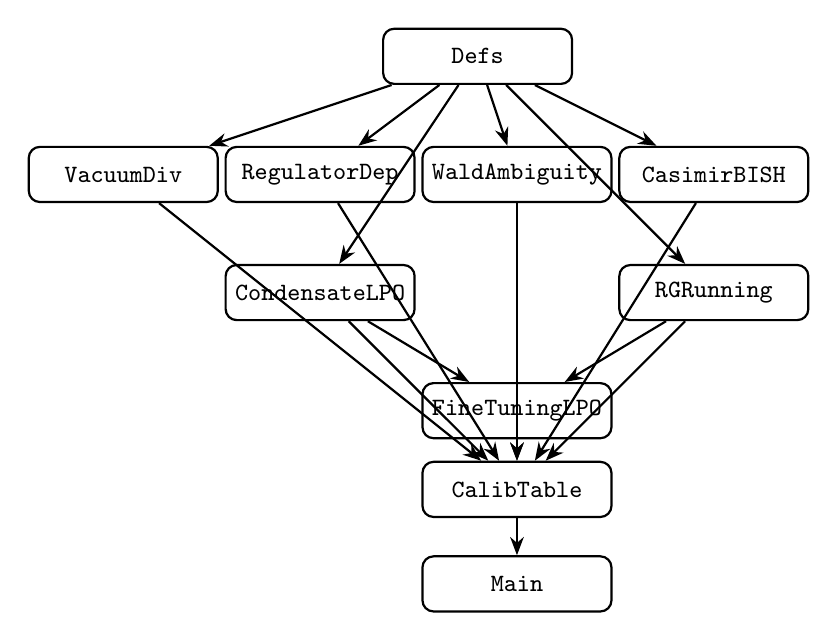
\begin{tikzpicture}[
  module/.style={draw, rounded corners, minimum width=2.4cm,
    minimum height=0.7cm, font=\small\ttfamily},
  ->,>=Stealth,thick
]
\node[module] (defs) at (0,6) {Defs};
\node[module] (vac) at (-4.5,4.5) {VacuumDiv};
\node[module] (reg) at (-2,4.5) {RegulatorDep};
\node[module] (wald) at (0.5,4.5) {WaldAmbiguity};
\node[module] (cas) at (3,4.5) {CasimirBISH};
\node[module] (cond) at (-2,3) {CondensateLPO};
\node[module] (rg) at (3,3) {RGRunning};
\node[module] (ft) at (0.5,1.5) {FineTuningLPO};
\node[module] (cal) at (0.5,0.5) {CalibTable};
\node[module] (main) at (0.5,-0.7) {Main};

\draw (defs) -- (vac);
\draw (defs) -- (reg);
\draw (defs) -- (wald);
\draw (defs) -- (cas);
\draw (defs) -- (cond);
\draw (defs) -- (rg);
\draw (cond) -- (ft);
\draw (rg) -- (ft);
\draw (vac) -- (cal);
\draw (reg) -- (cal);
\draw (wald) -- (cal);
\draw (cas) -- (cal);
\draw (ft) -- (cal);
\draw (cond) -- (cal);
\draw (rg) -- (cal);
\draw (cal) -- (main);
\end{tikzpicture}
\caption{Module dependency graph (10~modules, ${\sim}830$~lines).
  All seven theorem modules import \texttt{Defs}.
  \texttt{FineTuningLPO} imports both \texttt{CondensateLPO} and
  \texttt{RGRunningBISH}.  \texttt{CalibrationTable} imports all
  seven theorem modules.  \texttt{Main} imports only
  \texttt{CalibrationTable}.}
\label{fig:arch}
\end{figure}

% ====================================================================
\begin{mdframed}[linewidth=1pt, linecolor=black!40,
  backgroundcolor=blue!3, roundcorner=5pt]
\textbf{Reproducibility.}
\Lean{} v4.28.0-rc1 with \Mathlib{}.\\[3pt]
\textbf{Build:}
\begin{verbatim}
cd "paper 42/P42_CosmologicalConstant" && lake build
\end{verbatim}
\textbf{Result:} 0~errors, 0~warnings, 0~\texttt{sorry}.\\[3pt]
\textbf{Axiom audit:}
\begin{verbatim}
#print axioms cc_master
-- 'cc_master' depends on axioms:
-- [Lambda_obs, bmc_from_subadditive,
--  dimreg_value_different, eight_pi_G,
--  lattice_energy_bdd_below, lattice_energy_subadditive,
--  lattice_vacuum_energy, mode_sum_mono,
--  mode_sum_partial, mode_sum_unbounded,
--  picard_lindelof_lambda, propext,
--  regularized_vacuum_energy,
--  Classical.choice, Quot.sound]
\end{verbatim}
\textbf{Profile:} 12~unverified premises (11~physics bridge axioms +
1~CRM axiom) + 3~Lean infrastructure (\texttt{propext},
\texttt{Classical.choice}, \texttt{Quot.sound}).
The formalization verifies logical inferences from these premises,
not the premises themselves.\\[3pt]
\texttt{Classical.choice} is a Mathlib infrastructure artifact
(required by $\RR$ as a Cauchy completion);
constructive stratification is established by proof content
(explicit witnesses vs.\ principle-as-hypothesis), not by
axiom-checker output.  See Paper~10~\cite{Lee26P10}, \S Methodology.

\medskip\noindent
\textbf{Data availability.}
Source code and \LaTeX{} source are archived at
\href{https://doi.org/10.5281/zenodo.18654789}{doi:10.5281/zenodo.18654789}.
\end{mdframed}

% ====================================================================
\section{Conclusion}\label{sec:conclusion}

The cosmological constant problem, as usually stated, conflates
three logically distinct issues.  The axiom calibration framework
separates them:
\begin{enumerate}[nosep]
\item The $10^{120}$ is \textbf{dissolved}---it is a
  regulator-dependent artifact, not a prediction.
  The unregularized vacuum energy diverges (Theorem~\ref{thm:diverge});
  different regularizers give different finite values
  (Theorem~\ref{thm:regulator}).  There is no prediction.
\item Naturalness is \textbf{reclassified}---it is a Bayesian
  prior, not a theorem.  The Hollands--Wald axioms prove that the
  cosmological constant is a free parameter (Theorem~\ref{thm:wald}).
\item The 55-digit fine-tuning is \textbf{identified} as an
  $\LPO$ equality---real but logically mundane.  The exact condensates
  are $\LPO$-computable via Fekete (Theorem~\ref{thm:condensate});
  the equation holds by arithmetic (Theorem~\ref{thm:finetune}).
\end{enumerate}

The $\BISH + \LPO$ ceiling holds.  The cosmological constant problem
introduces no new logical resources beyond those already catalogued
in the programme.  $\LPO$ suffices for the fine-tuning equation, placing it at the
same level as the Ising model phase transition, the QCD confinement
scale, and every other thermodynamic limit in physics.

\medskip\noindent
\textbf{Significance.}\quad
Most papers in the programme classify known results: they identify
the constructive status of an established theorem (e.g., the
Heisenberg bound is $\BISH$, the Ising phase transition is $\LPO$).
This paper does something different.  It \emph{dissolves} a famous
problem: the ``worst prediction in physics'' is not a prediction.

The unregularized vacuum energy does not converge to a real number
at any level of the constructive hierarchy
(Theorem~\ref{thm:diverge}).  Different regulators produce
different finite values (Theorem~\ref{thm:regulator}).
The $10^{120}$ is a property of a calculational choice, not of
quantum field theory.  The Casimir effect
(Theorem~\ref{thm:casimir}) confirms that the scaffolding
diagnostic works: energy \emph{differences} are $\BISH$-computable
and experimentally verified; absolute vacuum energies are
regulator-dependent and physically meaningless.

The CRM analysis provides a formal, machine-checked expression
of the post-naturalness position articulated by
Martin~\cite{Martin2012}, Bianchi--Rovelli~\cite{BianchiRovelli2010},
and Hossenfelder~\cite{Hossenfelder2019}.  Where these authors
reached their conclusions through physical argumentation, the
present paper provides a type-theoretic formalization verified by
the Lean~4 proof assistant: the divergence, the regulator
dependence, and the free-parameter status of $\Lambda$ are each
machine-checked theorems.
The remaining genuine physics---the 55-digit fine-tuning---is
an $\LPO$ equality, logically mundane: the same level as every
thermodynamic limit in the programme.  The cosmological constant
problem requires no new logical resources.

% ====================================================================
\section{Discussion}\label{sec:discussion}

\subsection{What Is Dissolved}

The $10^{120}$ number is produced by cutoff regularization.
Dimensional regularization and $\zeta$-function regularization---which
preserve gauge and Lorentz invariance---produce qualitatively
different values.  The absolute vacuum energy depends on the choice
of regulator.  By the calibration framework's criterion
(empirical content must be scaffolding-invariant), the $10^{120}$
has no physical content.

The regulator dependence of the vacuum energy is not a novel
observation.  Martin~\cite{Martin2012} demonstrates pedagogically
that the quartic divergence $\sim \Lambda_{\mathrm{UV}}^4$ arises
only from hard-cutoff regularization, while dimensional
regularization removes all power-law divergences.  Bianchi and
Rovelli~\cite{BianchiRovelli2010} argue that $\Lambda$ should be
treated as a fundamental constant, not derived from microphysics.
What the CRM framework adds is a \emph{formal criterion} for
dissolution: the scaffolding diagnostic.  A quantity has empirical
content only if its value is invariant under change of mathematical
scaffolding (regularization scheme, basis, gauge).  The vacuum
energy fails this criterion---Theorem~\ref{thm:regulator} proves
it in Lean~4.  The CRM framework thus transforms an informal
physical intuition (``the $10^{120}$ is an artifact'') into a
machine-checked theorem with a precise logical status ($\BISH$).

The Casimir effect (Theorem~\ref{thm:casimir}) demonstrates the
correct pattern: energy \emph{differences} between configurations
are $\BISH$-computable and have been experimentally verified to
better than 5\%~precision~\cite{Lamoreaux1997}, with extensive
theoretical analysis in~\cite{Bordag2001,Casimir1948}.  Absolute
vacuum energies, by contrast, are regulator-dependent scaffolding.
The framework's dissolution is not merely formal: it tracks the
distinction that QFT itself makes between physically meaningful
differences and mathematically ambiguous absolutes.
To be precise: the dissolution targets the $10^{120}$ \emph{magnitude},
not the existence of vacuum energy contributions from individual
particle species.  Each massive species contributes $\sim m^4/(16\pi^2)$,
which is finite and $\BISH$-computable.  What is dissolved is the
narrative that summing these over all modes to the Planck scale
yields a ``prediction'' of $\MPl^4$---that step is
regulator-dependent and produces no invariant number.

\subsection{What Is Reclassified}

The Hollands--Wald axioms~\cite{HollandsWald2001,HollandsWald2005}
prove that $c_1$ (the cosmological constant)
is a free parameter of the renormalized theory.  The naturalness
argument---that $c_1$ ``should'' be of order $\MPl^4$---is a claim
about expected magnitudes, not a logical consequence.

The naturalness criterion originates with
't~Hooft~\cite{tHooft1980}, who proposed that a small parameter
is natural only if setting it to zero increases the symmetry.
The cosmological constant violates this criterion spectacularly:
no known symmetry protects a small $\Lambda$.
Burgess~\cite{Burgess2013} develops this observation into a
systematic effective field theory argument for why dark energy
is hard to derive from microphysics.

However, the naturalness criterion itself has faced sustained
criticism.  Hossenfelder~\cite{Hossenfelder2019} argues that
fine-tuning arguments require a probability distribution over
the parameter space, and no such distribution is derivable from
the theory; the arguments are therefore ``not scientifically
relevant'' in the absence of a measure.
Giudice~\cite{Giudice2017} diagnoses a broader ``post-naturalness
era,'' prompted in part by the LHC's failure to find new physics
at the electroweak scale.

The CRM framework provides a rigorous version of the
post-naturalness position.  Naturalness is not a theorem; it is
a claim about the expected magnitude of a free parameter.  Such
claims reside outside the $\BISH/\LPO$ deductive hierarchy because
they are not derivable from axioms---they are Bayesian priors.
The calibration framework can evaluate deductive structure, not
the plausibility of priors.

\subsection{What Is Identified}

The genuine constraint is the 55-digit cancellation between $\Lbare$
and the condensate contributions.  The exact condensates are
$\LPO$-computable via Fekete's lemma~\cite{Fekete1923,Lee26P29}.
The fine-tuning equation
\[
  \Lobs = \Lbare + 8\pi G\,(\rho_H^{\mathrm{exact}}
    + \rho_{\mathrm{QCD}}^{\mathrm{exact}})
\]
is an arithmetic relation between $\LPO$-computable reals.
The RG running above $\LQCD$ is $\BISH$ (Theorem~\ref{thm:rg});
below $\LQCD$, the non-perturbative QCD condensate brings the cost
to $\LPO$.

\begin{remark}[Upper bound, not tight equivalence]
The formalization establishes that $\LPO$ \emph{suffices} for
the fine-tuning equation---an upper bound on logical cost.
We do not prove the converse direction (that the fine-tuning
equation \emph{implies} $\LPO$).  Establishing a tight equivalence
(Fekete-style) would require constructing a binary sequence whose
$\LPO$-decidability is equivalent to the convergence of a specific
cosmological condensate---a direction left for future work.
The classification as ``$\LPO$'' should therefore be read as
``$\LPO$ suffices,'' consistent with the Fekete-based upper
bounds used throughout the programme.
Paper~29 establishes a provability equivalence (Fekete $\equiv$
$\LPO$ over $\BISH$); whether this lifts to a Weihrauch equivalence
in the sense of Brattka--Gherardi--Pauly~\cite{BrattkaEtAl2012}
is an open question that would further refine the computational
content of the fine-tuning equation.
\end{remark}

This decomposition connects to recent running vacuum
models~\cite{Sola2013}, which propose that the effective vacuum
energy density evolves with the Hubble rate via renormalization
group running.  In the CRM framework, the perturbative RG
running of these models is $\BISH$-computable (Picard--Lindel\"of
iteration on a Lipschitz ODE); the non-perturbative QCD condensate
contribution, which completes the picture, is where the $\LPO$
cost enters.  The BISH-to-LPO step is the same thermodynamic
limit that appears across the entire programme: it is not specific
to cosmology but is the generic logical cost of passing from
finite-volume approximations to infinite-volume exact values.

\subsection{What Is Not Explained}

The framework does not explain \emph{why} the cancellation occurs.
It identifies the \emph{logical status} ($\LPO$ equality), not the
\emph{physical cause}.

The string landscape~\cite{Polchinski2006,BoussoPolchinski2000}
provides one class of proposed explanations: the enormous number of
flux vacua (${\sim}10^{500}$) generates a dense discretuum of $\Lambda$
values, and anthropic selection picks a habitable one.  The CRM
framework does not address this: it identifies the logical structure
of the fine-tuning equation, not the selection mechanism that
determines its parameters.  Whether the cancellation arises from
an environmental selection (landscape), an unknown symmetry (SUSY),
a dynamical relaxation mechanism, or is simply a brute fact remains
an open physics question.

The preliminary DESI results~\cite{DESI2024} have introduced a further
complication: there are hints ($2.5$--$3.9\sigma$, depending on
data combination) that the dark energy equation of state evolves
in time ($w_0 > -1$, $w_a < 0$), which would mean $\Lambda$ is
not truly constant.  These results are preliminary and their
interpretation is debated in the literature; if confirmed by
future data releases, they would add a new dynamical
component to the problem.  In the CRM framework, the logical cost
of this additional component depends on its origin: perturbative
dynamics (e.g., a slowly rolling scalar field) would remain $\BISH$;
only if the dynamics involved a thermodynamic limit (e.g., a
condensate phase transition) would $\LPO$ enter.

\subsection{Relation to Other Approaches}

Nobbenhuis~\cite{Nobbenhuis2006} categorizes proposed solutions to
the cosmological constant problem into five classes:
(i)~symmetry mechanisms (SUSY, conformal symmetry, sequestering),
(ii)~back-reaction (vacuum energy screening by spacetime dynamics),
(iii)~modifications of general relativity (unimodular gravity,
degravitation),
(iv)~statistical/anthropic approaches (landscape plus selection),
and (v)~vacuum-energy adjustment mechanisms (relaxation, four-form
flux quantization).  The CRM analysis is orthogonal to all five:
it does not propose a mechanism but identifies the logical structure
of the quantities each mechanism must address.

Concretely: symmetry mechanisms aim to make $\Lambda$ naturally
small---this addresses the naturalness prior (Claim~II).  The CRM
framework classifies that prior as non-deductive rather than
refuting or endorsing it.  Back-reaction and GR modifications alter
the gravitational field equations; the CRM framework takes
Einstein's equations as given (bridge axioms).
Statistical/anthropic and adjustment approaches attempt to select
or explain the value of $\Lbare$; the CRM framework shows that
$\Lbare$ is a free parameter of the renormalized theory
(Theorem~\ref{thm:wald}, $\BISH$) and does not address the
selection question.

The closest connection is to running vacuum
models~\cite{Sola2013}: their perturbative renormalization group
running of the effective vacuum energy corresponds to Theorem~6
($\BISH$), and their non-perturbative contributions correspond
to Theorem~5 ($\LPO$).  The CRM framework thus provides a
logical stratification of the ingredients these models employ,
separating the computationally tractable (perturbative) from
the computationally expensive (thermodynamic limit).

\subsection{Connection to the Programme}

\textbf{Paper 10 (Logical Geography)~\cite{Lee26P10}:}\quad
Paper~10 assembles the complete calibration table---approximately
50~entries across 11~physical domains---and establishes the
certification methodology (mechanically certified, structurally
verified, intentionally classical).  The cosmological constant
problem adds approximately 12~new rows to this table.  The
$\BISH + \LPO$ ceiling continues to hold.

\textbf{Paper 12 (Constructive History)~\cite{Lee26P12}:}\quad
Paper~12 traces 150~years of non-constructive commitments in
mathematical physics, from Weierstrass's epsilon-delta analysis
through Boltzmann's thermodynamic limit.  The cosmological constant
problem is a paradigm case of Paper~12's thesis: the $10^{120}$
narrative involves layers of idealization (continuum limit,
naturalness prior) that the CRM framework can precisely locate
and, where appropriate, dissolve.

\textbf{Paper 29 (Fekete $\equiv$ LPO)~\cite{Lee26P29}:}\quad
The Fekete--LPO equivalence is the central mechanism.  The exact
vacuum condensates are subadditive (bridge axiom), and their
convergence costs $\LPO$ via Fekete's lemma---the same mechanism
governing the five previously identified $\LPO$ domains (statistical
mechanics, general relativity, decoherence, conservation laws,
quantum gravity).  This paper adds a sixth domain: vacuum QFT.

\textbf{Paper 33 (QCD Confinement)~\cite{Lee26P33}:}\quad
The non-perturbative QCD condensate $\rho_{\mathrm{QCD}}^{\mathrm{exact}}$
is the same thermodynamic limit studied in Paper~33's lattice QCD
formalization.  The confinement scale $\LQCD$ is $\LPO$-computable
for the same reason: the lattice free energy is subadditive.

\textbf{Paper 39 (Thermodynamic Stratification)~\cite{Lee26P39}:}\quad
The vacuum energy density is an extensive quantity.
By Paper~39's stratification theorem, extensive observables at full
precision cap at $\LPO$ (Fekete/BMC).  Intensive observables without
promise gaps can reach $\Sigma_2^0$ ($\LPO'$).  The CC problem stays
at $\LPO$ because all relevant quantities---energy densities,
condensates---are extensive.

\textbf{Paper 41 (AdS/CFT)~\cite{Lee26P41}:}\quad
In holographic theories, $\Lambda$ is determined by boundary CFT
data via the Brown--Henneaux relation ($\BISH$), suggesting that
in some UV completions the fine-tuning may be resolved by
consistency conditions rather than set by hand.

% ====================================================================
\section{AI-Assisted Methodology}\label{sec:ai}

This formalization was developed using Claude (Anthropic) as a
collaborative tool for \Lean{}~4 code generation, proof strategy
exploration, and \LaTeX{} document preparation.  All mathematical
content was specified by the author.  Every theorem was verified
by the \Lean{}~4 type checker.

\medskip\noindent
\textbf{Preliminary status and author background.}
The results presented in this paper are preliminary.  The author is a medical
professional, not a domain expert in physics or mathematics.  While all formal
claims are machine-checked by the \Lean{} type-checker, the physical
interpretations, bridge axioms, and modeling assumptions require independent
verification by domain experts.  Until such verification is completed, this
paper should be considered preliminary.

\medskip\noindent
Whatever findings of value emerge from this program belong to the
constructive reverse mathematics community and to the legacy of Errett Bishop,
whose perseverance in developing constructive analysis inspired this entire
series.  Any errors are solely the author's.

% ====================================================================
\begin{thebibliography}{35}

\bibitem{Weinberg1989}
S.~Weinberg,
``The cosmological constant problem,''
\emph{Reviews of Modern Physics} \textbf{61}(1), 1--23 (1989).

\bibitem{HollandsWald2001}
S.~Hollands and R.~M.~Wald,
``Local Wick polynomials and time ordered products of quantum fields
in curved spacetime,''
\emph{Communications in Mathematical Physics} \textbf{223}, 289--326 (2001).

\bibitem{HollandsWald2005}
S.~Hollands and R.~M.~Wald,
``Conservation of the stress tensor in perturbative interacting quantum
field theory in curved spacetimes,''
\emph{Reviews in Mathematical Physics} \textbf{17}, 227--311 (2005).

\bibitem{Casimir1948}
H.~B.~G.~Casimir,
``On the attraction between two perfectly conducting plates,''
\emph{Proceedings of the Koninklijke Nederlandse Akademie van Wetenschappen}
\textbf{51}, 793--795 (1948).

\bibitem{Fekete1923}
M.~Fekete,
``{\"U}ber die Verteilung der Wurzeln bei gewissen algebraischen Gleichungen,''
\emph{Mathematische Zeitschrift} \textbf{17}, 228--249 (1923).

\bibitem{Bishop1967}
E.~Bishop,
\emph{Foundations of Constructive Analysis},
McGraw-Hill (1967).

\bibitem{BridgesVita2006}
D.~Bridges and L.~Vita,
\emph{Techniques of Constructive Analysis},
Springer (2006).

\bibitem{BrattkaEtAl2012}
V.~Brattka, G.~Gherardi, and A.~Pauly,
``Weihrauch degrees, omniscience principles and weak computability,''
\emph{J.\ Symbolic Logic} \textbf{77}(1), 119--141 (2012).

\bibitem{Lee26P10}
P.~C.-K.~Lee,
``The logical geography of mathematical physics,''
Preprint, 2026. Paper~10.

\bibitem{Lee26P12}
P.~C.-K.~Lee,
``The map and the territory: a constructive history of
  mathematical physics,''
Preprint, 2026. Paper~12.

\bibitem{Lee26P29}
P.~C.-K.~Lee,
``Fekete's subadditive lemma is equivalent to LPO,''
Preprint, 2026. Paper~29.

\bibitem{Lee26P33}
P.~C.-K.~Lee,
``QCD one-loop renormalization and confinement: axiom calibration,''
Preprint, 2026. Paper~33.

\bibitem{Lee26P39}
P.~C.-K.~Lee,
``Beyond LPO: the thermodynamic stratification of physical undecidability,''
Preprint, 2026. Paper~39.

\bibitem{Lee26P40}
P.~C.-K.~Lee,
``Defending the $\BISH$+$\LPO$ characterization,''
Preprint, 2026. Paper~40.
\href{https://doi.org/10.5281/zenodo.18654773}{doi:10.5281/zenodo.18654773}.

\bibitem{Lee26P41}
P.~C.-K.~Lee,
``AdS/CFT and the constructive hierarchy,''
Preprint, 2026. Paper~41.
\href{https://doi.org/10.5281/zenodo.18654780}{doi:10.5281/zenodo.18654780}.

\bibitem{Zeldovich1968}
Ya.~B.~Zel'dovich,
``The cosmological constant and the theory of elementary particles,''
\emph{Soviet Physics Uspekhi} \textbf{11}(3), 381--393 (1968).

\bibitem{Riess1998}
A.~G.~Riess \emph{et al.},
``Observational evidence from supernovae for an accelerating universe
and a cosmological constant,''
\emph{The Astronomical Journal} \textbf{116}(3), 1009--1038 (1998).
arXiv:astro-ph/9805201.

\bibitem{Perlmutter1999}
S.~Perlmutter \emph{et al.},
``Measurements of $\Omega$ and $\Lambda$ from 42 high-redshift supernovae,''
\emph{The Astrophysical Journal} \textbf{517}(2), 565--586 (1999).
arXiv:astro-ph/9812133.

\bibitem{Planck2020}
Planck Collaboration,
``Planck 2018 results.\ VI.\ Cosmological parameters,''
\emph{Astronomy \& Astrophysics} \textbf{641}, A6 (2020).
arXiv:1807.06209.

\bibitem{DESI2024}
DESI Collaboration,
``DESI 2024 VI: Cosmological constraints from the measurements of
baryon acoustic oscillations,''
arXiv:2404.03002 (2024).

\bibitem{BridgesRichman1987}
D.~Bridges and F.~Richman,
\emph{Varieties of Constructive Mathematics},
London Mathematical Society Lecture Note Series~97,
Cambridge University Press (1987).

\bibitem{Ishihara2006}
H.~Ishihara,
``Reverse mathematics in Bishop's constructive mathematics,''
\emph{Philosophia Scientiae} CS~6, 43--59 (2006).

\bibitem{Carroll2001}
S.~M.~Carroll,
``The cosmological constant,''
\emph{Living Reviews in Relativity} \textbf{4}, 1 (2001).
arXiv:astro-ph/0004075.

\bibitem{Padmanabhan2003}
T.~Padmanabhan,
``Cosmological constant---the weight of the vacuum,''
\emph{Physics Reports} \textbf{380}(4--6), 235--320 (2003).
arXiv:hep-th/0212290.

\bibitem{Martin2012}
J.~Martin,
``Everything you always wanted to know about the cosmological constant
problem (but were afraid to ask),''
\emph{Comptes Rendus Physique} \textbf{13}(7), 566--665 (2012).
arXiv:1205.3365.

\bibitem{tHooft1980}
G.~'t~Hooft,
``Naturalness, chiral symmetry, and spontaneous chiral symmetry breaking,''
in \emph{Recent Developments in Gauge Theories},
NATO ASI Series~B, Vol.~59, Springer (1980), pp.~135--157.

\bibitem{Burgess2013}
C.~P.~Burgess,
``The cosmological constant problem: why it's hard to get dark energy
from micro-physics,''
in \emph{Post-Planck Cosmology: Les Houches 2013},
Oxford University Press (2015).
arXiv:1309.4133.

\bibitem{BianchiRovelli2010}
E.~Bianchi and C.~Rovelli,
``Why all these prejudices against a constant?''
arXiv:1002.3966 (2010).

\bibitem{Hossenfelder2019}
S.~Hossenfelder,
``Screams for explanation: finetuning and naturalness in the foundations
of physics,''
\emph{Synthese} \textbf{198}(Suppl.~16), 3727--3745 (2021).
arXiv:1801.02176.

\bibitem{Giudice2017}
G.~F.~Giudice,
``The dawn of the post-naturalness era,''
arXiv:1710.07663 (2017).

\bibitem{Nobbenhuis2006}
S.~Nobbenhuis,
``Categorizing different approaches to the cosmological constant problem,''
\emph{Foundations of Physics} \textbf{36}(5), 613--680 (2006).
arXiv:gr-qc/0411093.

\bibitem{BoussoPolchinski2000}
R.~Bousso and J.~Polchinski,
``Quantization of four-form fluxes and dynamical neutralization
of the cosmological constant,''
\emph{Journal of High Energy Physics} \textbf{2000}(6), 006 (2000).
arXiv:hep-th/0004134.

\bibitem{Polchinski2006}
J.~Polchinski,
``The cosmological constant and the string landscape,''
arXiv:hep-th/0603249 (2006).

\bibitem{Lamoreaux1997}
S.~K.~Lamoreaux,
``Demonstration of the Casimir force in the 0.6 to 6~$\mu$m range,''
\emph{Physical Review Letters} \textbf{78}(1), 5--8 (1997).

\bibitem{Bordag2001}
M.~Bordag, U.~Mohideen, and V.~M.~Mostepanenko,
``New developments in the Casimir effect,''
\emph{Physics Reports} \textbf{353}(1), 1--205 (2001).
arXiv:quant-ph/0106045.

\bibitem{Sola2013}
J.~Sol\`{a},
``Cosmological constant and vacuum energy: old and new ideas,''
\emph{J.\ Phys.\ Conf.\ Ser.}\ \textbf{453}, 012015 (2013).
arXiv:1306.1527.

\end{thebibliography}

\end{document}
